\chapter{Optimal Transport with Kernel-based Regularization}
\label{chap:ch1}

\section{Introduction}\label{sec:intro}
In this chapter, we propose and analyze the kernel-regularized OT formulations, where the marginal-matching constraints are enforced using kernel-based Maximum Mean Discrepancy (MMD) regularization.

The Kantorovich-OT formulation (Eq.~\ref{eqn:kot}), discussed in the previous chapter, strictly enforces the marginals of the transport plan to be the source and target measures. However, often, one prefers to relax this constraint when the empirical measures could be noisy~\citep{ROT} or when the source and target measures are unnormalized~\citep{chizat17,Liero2018}. We discussed $f$-divergence regularized OT formulations (Eq.~\ref{bgeqn:uot}) in the previous chapter, which employs $f$-divergence-based regularization terms for softly matching the transport plan's marginals with the source and the target distributions. Such variants have been studied under the name, Unbalanced Optimal Transport (UOT)~\citep{chizat17}.
UOT with KL-divergence (KL-OT)~\citep{Liero2016OptimalTI,Liero2018} and, in general, with $f$-divergence~\citep{Csiszar67} based regularization is well-explored in literature. 
With an additional entropy regularization, the resulting formulation ($\epsilon$-KLOT) enjoys scalable solvers based on the Sinkhorn algorithm~\citep{ChizatPSV18,chizat18a}. There has been a diverse set of applications~\citep{jumbot,ijcai2020p516,De_Plaen_2023_CVPR} where $\epsilon$-KLOT has enormously improved the performance compared to the Kantorovich-OT formulation.
Existing works~\citep{Piccoli2014GeneralizedWD,pic2016,tvdual,4689383} have also studied UOT formulations with regularization based on Total Variation (TV), another member of the $f$-divergence family, though TV-regularized UOT (TV-OT) is computationally less efficient as its optimization requires solving a Linear Program.

Our work is motivated by the observation that the regularized variants of OT have focused on regularizations based on $f$-divergences. These variants are primarily formulated to extend the applicability of Kantorovich-OT to unnormalized/unbalanced measures or to provide robustness guarantees. The focus in these regularized variants of OT has not been on improving the statistical aspects (Sec.~\ref{bg:ot-stats}) of the Kantorovich-OT formulation. We first observe that metrics like MMD, which belong to the class of Integral Probability Metrics (IPMs), exhibit statistical efficiency (Sec.~\ref{bg:kernel-stats}) and have been successfully applied in various ML applications~\citep {gretton12a,Li17,Li21,nguyen20}. However, the role of using such functions as regularizers in the OT formulations seems less understood. To bridge this gap, we propose and analyze the family of MMD-regularized OT (MMD-OT) formulations and later show that most of our results also extend to the family of IPM-regularized OT.

% We begin by deriving a specific dual of MMD-regularized OT (MMD-OT), which helps us prove several useful properties. 
% One interesting outcome of this duality result is that MMD-OT induces novel metrics, which not only lift the ground metric like the Wasserstein but are also sample-wise efficient to estimate like the MMD. 
% Further, for real-world applications involving non-discrete measures, we present an estimator for the transport plan that is supported only on the given ($m$) samples.
% Under certain conditions, we prove that the estimation error with this finitely-supported transport plan is also $O(1/\sqrt{m})$. To the best of our knowledge, such error bounds that are free from the curse of dimensionality are not known for $f$-divergence regularized OT. Finally, we discuss how the proposed estimator can be computed efficiently using an accelerated variant of gradient descent. Our proposed approach also extends to the case of unnormalized measures. 


We first derive a specific dual of the MMD-OT formulation (Theorem~\ref{thm:dual}), which helps further analyze its properties. One interesting consequence of this duality result is that the optimal objective of MMD-OT is a valid distance between the source and target measures (Corollary~\ref{corr:ipm}) whenever the cost function is a valid metric over the support. Popularly, this is known as the phenomenon of lifting ground metrics to that over the measures. This result is significant as it shows that MMD-regularization in OT can parallel the metricity-preservation that happens with KL-regularization~\citep{Liero2018} and TV-regularization~\citep{Piccoli2014GeneralizedWD}. Furthermore, our duality result shows that the metric induced by MMD-OT belongs to the family of Integral Probability Metrics (IPMs) with a generating set that is the intersection of the generating sets of MMD and the Kantorovich-Wasserstein metric. Owing to this important relation, the proposed distance is always smaller than a (scaled) MMD distance, and hence, estimating MMD-OT from samples is at least as efficient as that with MMD~(Corollary~\ref{corr:sampcomp}). This is interesting as minimax estimation rates for MMD can be completely dimension-free. To the best of our knowledge, there are no such results that show that estimation with KL/TV-regularized OT can be as efficient sample-wise. Thus, the proposed metrics not only lift the ground metrics to measures, like the Wasserstein but also are sample-wise efficient to estimate, like MMD. Our result of MMD-OT being a metric is especially useful for applications where the metric properties of OT are desired, for example, while computing the barycenter-based interpolation for single-cell RNA sequencing~\citep{TNet20}. 

We now highlight aspects of efficient estimation of our metrics. Like any OT formulation, the computation of MMD-OT involves optimization over all possible joint measures. This may be challenging, especially when the measures are continuous. To tackle this, we present a convex program-based estimator, which only involves a search over joints supported at the samples. We prove that the proposed estimator is statistically consistent and converges to MMD-OT between the true measures at a rate $O\left(m^{-\frac{1}{2}}\right)$, where $m$ is the number of samples. Such efficient estimators are particularly useful in ML applications, where typically only samples from the underlying measures are available. 
In contrast, the minimax estimation rate for the Wasserstein distance is itself $O\left(m^{-\frac{1}{d}}\right)$, where $d$ is the dimensionality of the samples~\citep{dudley1969,nilesweed2019estimation}. That is, even if a search over all possible joints is performed, estimating Wasserstein may be challenging. Since the proposed MMD-OT can approximate Wasserstein arbitrarily closely (as the regularization hyperparameter goes $\infty$), our result can also be understood as a way of alleviating the curse of dimensionality problem in Wasserstein.
Accordingly, we also present a finite-dimensional convex-program-based estimator for the barycenter with MMD-OT. We prove that this estimator is also consistent with an efficient sample complexity. We discuss how the formulations for estimating MMD-OT (and barycenter) can be solved efficiently using accelerated (projected) gradient descent. This solver helps us scale to large datasets. We empirically show the utility of MMD-OT in several applications, including two-sample hypothesis testing, single-cell RNA sequencing, domain adaptation, and prompt learning for few-shot classification, where MMD-OT outperforms related divergences and popular application-specific baselines.
\section{Contributions}
We summarize our main contributions as follows.
\begin{itemize}
    \item We derive and analyze the dual of the proposed MMD-regularized OT (MMD-OT). Using this result, we prove that MMD-OT induces novel metrics belonging to the family of IPMs that not only lift ground metrics like the Wasserstein but also are sample-wise efficient to estimate like the MMD.
    \item We propose finite-dimensional convex-program-based estimators for MMD-OT and the corresponding barycenter. We prove that these estimators are both statistically and computationally efficient.
    \item We illustrate the efficacy of MMD-OT in several real-world applications. Empirically, we observe that MMD-OT consistently outperforms related divergences and popular application-specific baselines. 
\end{itemize}
    We present proofs for all our theory results in Appendix~\ref{App:proofs}. It is noteworthy that most of our results not only hold for MMD-OT but also for a general family of IPM-regularized OT. Proofs in the appendix are hence written with a general IPM-based regularization and then specialized to the case when the IPM is MMD. This generalization to IPMs may itself be of independent interest.

\begin{table}[t]
\caption[Summarizing theoretical comparison of the proposed MMD-OT metric with other kernel and OT-based divergences.]{Comparing the proposed MMD-OT metric with other kernel and OT-based divergences. $\epsilon$-OT and $\epsilon$-KLOT denote the entropy-regularized scalable variants of OT and KL-OT, respectively.}\label{table:comp}
% \begin{center}
\centering
\setlength{\tabcolsep}{0.3em}
\small
\begin{tabular}{lccccccc}
\toprule
 Property &   MMD & OT & $\epsilon$-OT & TV-OT & KL-OT& $\epsilon$-KLOT &  \cellcolor{green!10}Proposed\\
  &  &  &  &  &  &  & \cellcolor{green!10}(MMD-OT)\\
\midrule
 Metricity & \tikzcmark & \tikzcmark & \tikzxmark & \tikzcmark & \tikzcmark & \tikzxmark & \tikzcmark\\
 Lifting of ground metric &  \tikzxmark & \tikzcmark & \tikzcmark & \tikzcmark & \tikzcmark & \tikzcmark  & \tikzcmark \\
 No C.O.D. & \tikzcmark & \tikzxmark & \tikzxmark & \tikzxmark & \tikzxmark  & \tikzxmark  & \tikzcmark\\
Bounds with finitely- & \multirow{2}{*}{N/A} & \multirow{2}{*}{\tikzxmark} & \multirow{2}{*}{\tikzxmark} & \multirow{2}{*}{\tikzxmark} & \multirow{2}{*}{\tikzxmark}  & \multirow{2}{*}{\tikzxmark}  & \multirow{2}{*}{\tikzcmark}\\
parametrized plan   &  &  &  &  &  &  & \\
Alignment over supports  &  \tikzxmark & \tikzcmark & \tikzcmark & \tikzcmark & \tikzcmark & \tikzcmark  & \tikzcmark \\
With unnormalized measures & \tikzcmark & \tikzxmark & \tikzxmark & \tikzcmark & \tikzcmark & \tikzcmark & \tikzcmark\\
\bottomrule
\end{tabular}
% \end{center}
\end{table}
\section{Preliminaries for the Chapter}\label{sec:background}
We begin by recalling relevant notations and then discuss the relevant background materials for this chapter.
\paragraph{Notations.} $\calX$ denotes a domain for the supports that forms a compact Hausdorff space. $\calR^+(\calX)$ and $\calR(\calX)$ denote the set of all non-negative, signed (finite) Radon measures defined over $\calX$; while the set of all probability measures is denoted by $\calR^+_1(\calX)$. $\sigma_1, \ \sigma_2$ denote the net masses of the two measures. For a measure, $\pi\in\calR^+(\calX\times\calX)$, on the product space, $\pi_1$ and $\pi_2$ denote the first and second marginals, respectively (i.e., they are the push-forwards under the canonical projection maps onto $\calX$). $\calL(\calX)$, $\calC(\calX)$ denotes the set of all real-valued measurable functions and all real-valued continuous functions, respectively, over $\calX$.
\newline We recall the definition of MMD as follows.
Let $\|f\|_k$ denote the norm of $f$ in the RKHS, $\calH_k$, corresponding to $k$. Using a characteristic kernel $k$, MMD between $s_0, t_0\in \calR^+(\calX)$ is defined as:
\begin{align}\label{uot:mmd}
    \MMD_k(s_0,t_0)&\equiv  \max\limits_{f\in\calG_k}\left|\int_\calX f\ \textup{d}s_0-\int_\calX f\ \textup{d}t_0\right|\nonumber\\
     &= \|\mu_k\left(s_0\right)-\mu_k\left(t_0\right)\|_k,
\end{align}
where $\mu_k\left(s\right)\equiv \E_{X\sim s}\left[\phi_k(X)\right]$, is the Kernel Mean Embedding of $s$ with $\phi_k$ as the feature map of $k$ and $\calG_k\equiv\left\{f\in\calH_k |\ \|f\|_k\le1\right\}$. We will use the notation MMD when the properties specific to the use of kernel $k$ are not being discussed. Given the samples from the two measures, the MMD metric can be computed in closed form using the evaluations of the kernel function (Sec.~\ref{bg:kernel-comp}).
\newline
We now present other preliminaries for this chapter.
\subsection{Integral Probability Metric}
\begin{definitionBox}
\begin{definition}{\textbf{Integral Probability Metric.}}\newline
Given a set $\calG\subset\calL(\calX)$, the Integral Probability Metric (IPM)~\citep{mullergenset97,Sriperumbudur09onintegral,agrawal20a} associated with $\calG$, is defined by:
\begin{equation}\label{eqn:ipm}     I_\calG(s_0,t_0)\equiv\max\limits_{f\in\calG}\left|\int_\calX f\ \textup{d}s_0-\int_\calX f\ \textup{d}t_0\right|\ \forall\ s_0,t_0\in\calR^+(\calX).
\end{equation}
$\calG$ is called the generating set of the IPM, $ I_\calG$.
\end{definition}
\end{definitionBox}
 $\MMD_k$ is the IPM associated with the generating set: $\calG_k\equiv\left\{f\in\calH_k |\ \|f\|_k\le1\right\}$. The other IPMs that appear in our theoretical results are defined below.
\paragraph{Kantorovich Metric.}
\begin{definitionBox}
\begin{definition}{\textbf{Kantorovich Metric.}}\newline
Kantorovich metric ($\mathcal{K}_c$) is an integral probability metric associated with the generating set $\calW_c\equiv \left\{ f:\calX\mapsto \mathbb{R} ~|~ \max\limits_{x\in\calX\neq y\in\calX} \frac{|f(x)-f(y)|}{c(x, y)} \leq 1 \right\}$, where $c$ is a metric over $\calX \times \calX$.  
\end{definition}
\end{definitionBox}
The Kantorovich-Rubinstein duality result shows that the 1-Wasserstein metric is the same as the Kantorovich metric when restricted to probability measures (\citep[(5.11)]{villanioldnew}). For $s_0,\ t_0\in\calR^+_1(\calX)$, we have the following,
\begin{align*}\label{eqn:koteqdual}
\bar{W}_{c,1}(s_0,t_0)&\ \ \equiv&\min\limits_{\pi\in\calR^+_1(\calX\times\calX)}\int c^p\ \textup{d}\pi, &\ \ =\ &\max\limits_{f\in\calW_c}\left|\int_\calX f\ \textup{d}s_0-\int_\calX f\ \textup{d}t_0\right|&\ \ \equiv&\calK_c(s_0,t_0),\\
&&\textup{ s.t.}\ \ \pi_1=s_0,\ \pi_2=t_0.
\end{align*}
\paragraph{Total Variation Metric.}
\begin{definitionBox}
    \begin{definition}{\textbf{Total Variation Metric.}}\newline
        Total Variation (TV) is an integral probability metric associated with the generating set: $\mathcal{T}\equiv\left\{f:\calX\mapsto\R\ |\ \|f\|_\infty\le1\right\},$ where $\|f\|_\infty\equiv\max\limits_{x\in\calX}|f(x)|$. Total Variation metric over measures $s_0, t_0\in \calR^+(\calX)$ is defined as:
\vspace{-0.17in}
\begin{equation*}\textup{TV}(s, t)\equiv \int_{\calY} \textup{d} |s-t|(y)\textup{, where }|s-t|(y)\equiv\Bigg\{\begin{array}{cc}
    s(y)-t(y) & \textup{if } s(y)\ge t(y) \\
    t(y)-s(y) & \textup{otherwise}
\end{array}.        
\end{equation*}
    \end{definition}
\end{definitionBox}

% \subsection{Dudley Metric}
% \begin{definitionBox}
%     \begin{definition}{\textbf{Dudley Metric.}}\newline
%         Dudley metric is an integral probability metric associated with the generating set:\\ $\calD_d\equiv\left\{f:\calX\mapsto\R\ |\ \|f\|_\infty+\|f\|_d\le1\right\},$ where $d$ is a ground metric over $\calX \times \calX$. The so-called \textbf{Flat} metric, related to the Dudley metric, is again an IPM with its generating set as $\mathcal{F}_d\equiv\left\{f:\calX\mapsto\R\ |\ \|f\|_\infty\le1,\|f\|_d\le1\right\}$.
%     \end{definition}
% \end{definitionBox}

Another popular IPM we refer to in our work is the Dudley metric. Dudley metric is an IPM associated with the generating set: $\calD_d\equiv\left\{f:\calX\mapsto\R\ |\ \|f\|_\infty+\|f\|_d\le1\right\},$ where $d$ is a ground metric over $\calX \times \calX$.
The Flat metric, related to the Dudley metric, is again an IPM with its generating set as $\mathcal{F}_d\equiv\left\{f:\calX\mapsto\R\ |\ \|f\|_\infty\le1,\|f\|_d\le1\right\}$.

\subsection{Some Characterizations of Functions}
We present some characterizations of functions that will be used to devise an efficient solver for the proposed estimator of the MMD-OT optimization problem.
\begin{definitionBox}
\begin{definition}{\textbf{Lipschitz Function.}}\label{defn:f-L}\newline
A function $f: \R^d\mapsto \R$ is said to Lipschitz continuous with constant $L$ (or $L$-Lipschitz) iff $\forall \mathbf{x}, \mathbf{y} \in \R^d$, the following inequality holds,
$$|f(\mathbf{x})-f(\mathbf{y})|\leq L\|\mathbf{x}-\mathbf{y}\|_2.$$
\vspace{-0.4in}
\end{definition}
\end{definitionBox}

\begin{definitionBox}
\begin{definition}{\textbf{Smooth Function.}}\label{defn:f-L-smooth}\newline
A differentiable function $f: \R^d\mapsto \R$ is said to smooth with smoothness constant $L$ (or $L$-smooth) iff $\forall \mathbf{x}, \mathbf{y}\in \R^d$, the following inequality holds,
\begin{equation*}
    f(\mathbf{y})-f(\mathbf{x}) + \langle \nabla f(\mathbf{x}), \ \mathbf{y}-\mathbf{x} \rangle \leq \frac{L}{2}\|\mathbf{x}-\mathbf{y}\|^2.
    %\label{f-L-smooth}
\end{equation*}
\end{definition}
\end{definitionBox}
An equivalent criterion for a differentiable function $f$ to be $L$-smooth is its gradient, $\nabla f$, being $L$-Lipschitz.

\section{Literature Review}\label{sec:related}
Prior works have studied $ f$-divergence-based regularization in the OT formulation, popularly known as unbalanced OT (UOT)  formulations~\citep{Liero2018,chizat18a}. The $f$-divergence regularized UOT formulation \citep{chizat17} may be written as follows.
\begin{equation}\label{eqn:kl}
\min\limits_{\pi\in\calR^+\left(\calX\times\calX\right)}\ \int c\ \textup{d}\pi + \lambda D_\phi(\pi_1,s_0) + \lambda D_\phi(\pi_2,t_0),
\end{equation}
where $c$ is the ground cost metric and $D_\phi(\cdot,\cdot)$ denotes the $f$-divergence~\citep{Csiszar67,Sriperumbudur09onintegral} between two measures. 

UOT with KL-divergence-based regularization (KL-OT) induces the so-called Gaussian Hellinger-Kantorovich metric~\citep{Liero2018} between the measures whenever $0<\lambda\leq 1$ and the ground cost $c$ is the squared-Euclidean distance.
An additional entropy regularization in KL-OT formulation facilitates Sinkhorn iteration~\citep{knight08a} based efficient solver for KL-OT~\citep{ChizatPSV18} and has been popularly employed in several ML applications~\citep{jumbot, ijcai2020p516,arase-etal-2023-unbalanced, De_Plaen_2023_CVPR}.

UOT with TV-divergence-based regularization (TV-OT) induces the so-called Generalized Wasserstein metric~\citep{Piccoli2014GeneralizedWD} between the measures whenever $\lambda>0$ and the ground cost $c$ is a valid metric. To the best of our knowledge, there are no scalable solvers to estimate the metrics induced by TV-OT formulation.

Besides the family of $f$-divergences, the family of Integral Probability Metrics (IPMs) is popularly used for comparing measures. An important member of the IPM family is the MMD metric, which also incorporates the geometry over supports through the underlying kernel. Due to its attractive statistical properties~\citep{Gretton06twosample}, MMD has been successfully applied in a diverse set of applications, including hypothesis testing~\citep{gretton12a}, generative modeling~\citep{Li17}, self-supervised learning~\citep{Li21}, etc. 

There are some key differences between MMD and OT-based approaches. 
A distinguishing feature of OT-based approaches is the feature of lifting the ground-metric geometry to that over distributions. 
One such result is visualized in Fig.~\ref{fig:planbarytime}(b), where the MMD-based-interpolate of the two unimodal distributions comes out to be bimodal. This is because MMD's interpolation is the (empirical) average of the source and the target densities, irrespective of the kernel. This has been well-established in the literature \citep{bottou2017geometrical}. On the other hand, OT-based approaches obtain a uni-modal barycenter. This is a `geometric' interpolation that captures the characteristic aspects of the source and the target distributions. 
Another feature of OT-based methods is that we obtain a transport plan between the source and the target points, which can be used for various alignment-based applications, e.g., cross-lingual word mapping~\citep{alvarez18wordEmb}, domain adaptation \citep{courty17b,Courty17domAda}, etc. On the other hand, it is unclear how MMD can be used to align the source and target data points.

This calls for an integration of OT and MMD-based approaches.
Recently,~\cite{ot-kme} explored learning the transport plan’s Kernel Mean Embeddings for the OT formulation (over normalized measures). 
The authors proposed learning the Kernel Mean Embedding of a joint distribution that incurs the least expected cost and whose marginal embeddings are close to the given-sample-based estimates of the marginal embeddings. 
As Kernel Mean Embedding are compared with MMD distance, MMD-based regularization features in the formulation of~\cite{ot-kme} as a means to control overfitting. To ensure that valid conditional embeddings are obtained from the learned joint embeddings,~\cite{ot-kme} required additional feasibility constraints restricting their solvers in scaling well to ML applications.
We also note that~\cite{ot-kme} neither analyze the dual of their formulation nor study its metric-related properties, and their sample complexity result of $O(m^{-\frac{1}{2}})$ does not apply to our MMD-OT estimator as their formulation is different from the proposed MMD-OT formulation (\ref{eqn:proposed}).
In contrast, we bypass the issues related to the validity of conditional embeddings as our formulation involves directly learning the transport plan and avoids learning the Kernel Mean Embedding of the transport plan. 
We perform a detailed study of MMD regularization for OT, which includes analyzing its dual and proving metric properties that are crucial for optimal transport formulations. 
To the best of our knowledge, the metricity of MMD-regularized OT formulations has not been studied previously. The proposed algorithm scales well to large-scale machine learning applications. 
While we also obtain $O(m^{-\frac{1}{2}})$ estimation error rate, we require a different proof strategy than~\cite{ot-kme}. Finally, as discussed in Appendix~\ref{App:proofs}, most of our theoretical results apply to a general IPM-regularized OT formulation and are not limited to the MMD-regularized UOT formulation. This generalization does not hold for~\cite{ot-kme}.

Finally, we differentiate our contributions from Wasserstein auto-encoders (WAE), which also employ MMD for regularization. The regularization in WAEs is only performed for one of the marginals, and the other marginal is matched exactly. This not only breaks the symmetry (and hence the metric properties) but also brings back the curse of dimensionality in estimation (for the same reasons as with unregularized OT). Further, their work does not attempt to study any theoretical properties with MMD regularization and merely employs it as a practical tool for matching marginals. We aim to theoretically study the metric and estimation properties with MMD regularization in OT.

We summarize the comparison between MMD-OT and relevant OT variants in Table~\ref{table:comp}.
\section{Proposed Methodology}\label{sec:main}
In this section, we present our proposed MMD-regularized OT formulation, discuss its theoretical properties, present finite-sample-based estimators highlighting their statistical and computational properties and finally, present and analyze the proposed barycenter obtained with our OT formulation.
\subsection{Proposed Formulation of MMD-OT}
Our proposed OT formulation with marginals softly matched using kernel-based MMD regularization is presented below.
\begin{definitionBox}
\vspace{-0.15in}
\begin{align}\label{eqn:proposed}
\calU\left(s_0,t_0\right)&\equiv\min\limits_{\pi\in\calR^+\left(\calX\times\calX\right)} \int c ~\textup{d}\pi + \lambda_1 \MMD_k(\pi_1, s_0) 
    + \lambda_2 \MMD_k(\pi_2, t_0) \nonumber\\
    &= \min\limits_{\pi\in\calR^+\left(\calX\times\calX\right)} \int c ~\textup{d}\pi + \lambda_1 \|\mu_k\left(\pi_1\right)-\mu_k\left(s_0\right)\|_k+ \lambda_2 \|\mu_k\left(\pi_2\right)-\mu_k\left(t_0\right)\|_k,
\end{align}
where $s_0$ and $t_0\in \calR^+(\calX)$, $\mu_k(s)$ is the Kernel Mean Embedding of $s$ with the characteristic kernel $k$ and $\Lambda=\{\lambda_1,\ \lambda_2\}$; $\lambda,\ \lambda_2>0$.
\end{definitionBox}

\noindent We present the theoretical properties of MMD-OT beginning with a key duality result.
\subsection{Duality and Metricity}
This section presents our key theorem on the dual of MMD-OT. The subsequent corollaries in this section and Sec.~\ref{uot:sampc} present the desirable properties of our formulation that follow from this result.
\begin{theoremBox}
\begin{theorem}[Dual of MMD-OT]\label{thm:dual}
 Whenever $c, k\in\calC(\calX\times\calX)$ and $\calX$ is compact, our duality result gives the following.
 \begin{align}\label{uot-eqn:dual}
\calU\left(s_0,t_0\right)=\max\limits_{f\in\calG_k(\lambda_1),g\in\calG_k(\lambda_2)}&\int_\calX f\ \textup{d}s_0+\int_\calX g\ \textup{d}t_0, \nonumber\\
    &\textup{s.t. }f(x)+g(y)\le c(x,y)\ \forall\ x,y\in\calX.
 \end{align}
% \begin{equation}
% \begin{array}{ll}
%     \calU\left(s_0,t_0\right)=&\max\limits_{f\in\calG_k(\lambda_1),g\in\calG_k(\lambda_2)}\int_\calX f\ \textup{d}s_0+\int_\calX g\ \textup{d}t_0,\\
%     &\ \ \ \ \ \ \ \ \ \textup{s.t.}\ \ \ \ \ \  f(x)+g(y)\le c(x,y)\ \forall\ x,y\in\calX.
% \end{array}
% \end{equation}
Here, $\calG_k(\lambda)\equiv\{g\in \calH_k\ |\ \|g\|_k\le\lambda\}$.
\end{theorem}
\end{theoremBox}

The duality result helps us to study several properties of MMD-OT (\ref{eqn:proposed}) which we discuss in the following corollaries. The proof of Theorem~\ref{thm:dual} is based on an application of Sion's minimax exchange theorem~\citep{Sion} and is detailed in Appendix~\ref{proof:thm-dual}.

Applications in ML often involve comparing distributions for which the Wasserstein metric is a popular choice. While prior works have shown metric-preservation happens for OT formulations with KL-regularization~\citep{Liero2018} and TV-regularization~\citep{pic2016}, it is an open question if MMD-regularization in UOT also leads to valid metrics. Our following result answers this affirmatively.
\begin{corollaryBox}
\begin{corollary}[Metricity of MMD-OT]\label{corr:ipm} 
In addition to assumptions in Theorem (\ref{thm:dual}), whenever $c$ is a metric and $\lambda_1=\lambda_2$, we have the following.
\begin{itemize}
    \item $\calU$ belongs to the family of Integral Probability Metrics (IPMs).
    \item The generating set of this IPM is the intersection of the generating set of the Kantorovich metric and the generating set of MMD.
    \item $\calU$ is a valid norm-induced metric over measures whenever $k$ is characteristic. Thus, $\calU$ \emph{lifts} the ground metric $c$ to that over measures.
\end{itemize}
\end{corollary}
\end{corollaryBox}
The proof of Corollary~\ref{corr:ipm} is detailed in Appendix~\ref{proof:corr-metricity}.

Corollary~\ref{corr:ipm} shows a relation between the generating sets of the Kantorovich metric, the MMD metric and the metrics induced by MMD-OT.
The duality result also reveals interesting relationships between $\calU$, the Kantorovich metric ($\calK_c$) and the MMD metric used for regularization. This is summarized in the next two corollaries. For simplicity of notations, we will continue to assume $\lambda_1=\lambda_2=\lambda$, unless stated otherwise.
\begin{corollaryBox}
\begin{restatable}[MMD-OT interpolates between Kantorovich and MMD]{corollary}{interpolant}
\label{interp} In addition to assumptions in Corollary~\ref{corr:ipm}, if the kernel is c-universal (continuous and universal), then $\forall\ s_0,t_0\in\calR^+(\calX)$, we have $\lim_{\lambda\rightarrow\infty}\calU(s_0,t_0)=\calK_c(s_0,t_0)$.  

Further, if the cost metric, $c$, dominates the characteristic kernel, $k$, induced metric, i.e., $c(x,y)\ge\sqrt{k(x,x)+k(y,y)-2k(x,y)}\ \forall\ x,y\in\calX$, then $\ \calU(s_0, t_0)=\lambda \MMD_k(s_0, t_0)$ whenever $0<\lambda\leq 1$. Finally, when $\lambda\in(0,1)$, MMD-OT interpolates between the scaled MMD and the Kantorovich metric.
\end{restatable}
\end{corollaryBox}
\begin{figure}[t]
\centering
\begin{subfigure}{.3\textwidth}
    \centering
    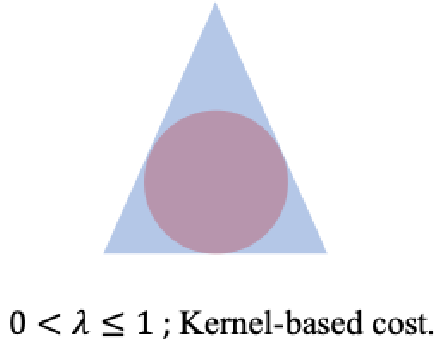
\includegraphics[scale=0.5]{chapter-1/images/metric1.pdf}  
    \caption{MMD}
    %\label{sim1}
\end{subfigure}
\begin{subfigure}{.3\textwidth}
    \centering
    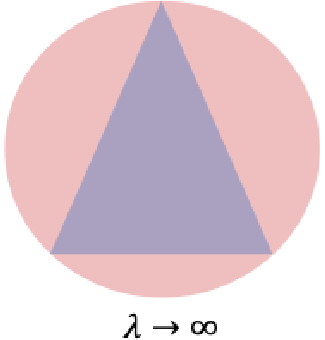
\includegraphics[scale=0.5]{chapter-1/images/metric2.pdf}  
    \caption{Kantorovich}
    %\label{sim1}
\end{subfigure}
\begin{subfigure}{.3\textwidth}
    \centering
    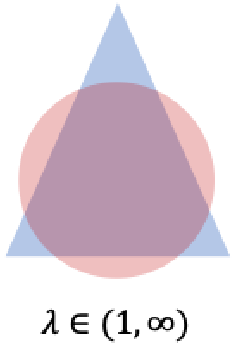
\includegraphics[scale=0.5]{chapter-1/images/metric3.pdf}  
    \caption{Proposed novel metrics}
    %\label{sim1}
\end{subfigure}
\caption[Illustration of the generating set of the proposed MMD-OT metric.]{Illustration of the generating set of the proposed MMD-regularized OT metric. The generating set of Kantorovich-Wasserstein is depicted as a triangle, and the scaled generating set of MMD is depicted as a disc. The intersection represents the generating set of the IPM metric induced by MMD-OT. (a) shows the special case when our MMD-OT metric recovers back the sample-efficient MMD metric, (b) shows the special case when our MMD-OT metric reduces to the Kantorovich-Wasserstein metric that lifts the ground metric to measures, and (c) shows the family of novel metrics which are both sample-efficient like MMD and can lift ground metrics to measures like Wasserstein.}\label{fig:metric}
\end{figure}


We illustrate this interpolation result in Fig.~\ref{fig:metric}. Our proof of Corollary~\ref{interp}, presented in Appendix~\ref{proof:corr-interp}, also substantiates the dominating cost assumption by showing with the Euclidean distance when the kernel employed is the Gaussian kernel and the inputs lie on a unit-norm ball.

\subsection{Sample Complexity and Some Additional Results}\label{uot:sampc}
 We now show that the sample complexity of the metric induced by MMD-OT resembles the dimension-free statistical efficiency of the MMD metric. In typical ML applications, only finite samples are given from the measures. Hence, it is important to study statistically efficient metrics that alleviate the curse of dimensionality problem prevalent in popular  OT variants~\citep{nilesweed2019estimation}.

 We begin by showing an interesting relationship between the proposed MMD-OT metric, Kantorovich metric and the MMD metric, which is again a consequence of our duality result (Theorem~\ref{thm:dual}).
 \begin{corollaryBox}
 \begin{corollary}[Relation between MMD-OT, Kantorovich Metric and MMD]\label{corr:rel}
    $\calU(s_0, t_0)\leq \min\left(\lambda\MMD_k(s_0, t_0),\ \calK_c(s_0, t_0)\right).$
\end{corollary}
 \end{corollaryBox}
The proof of Corollary~\ref{corr:rel} is straightforward and is presented in Appendix~\ref{proof:corr}. This result enables us to show properties like weak metrization and sample efficiency with MMD-OT. For a sequence $s_n\in \calR_1^+(\calX), ~n\geq 1$, we say that $s_n$ weakly converges to $s\in \calR_1^+(\calX)$ (denoted as $s_n\rightharpoonup s$), if and only if $~\mathbb{E}_{X\sim s_n}[f(X)]\rightarrow\mathbb{E}_{X\sim s}[f(X)]$ for all bounded continuous functions over $\calX$. It is natural to ask when is the convergence in metric over measures equivalent to weak convergence on measures. The metric is then said to metrize the weak convergence of measures or is equivalently said to weakly metrize measures. The weak metrization properties of the Wasserstein metric and MMD are well-understood (e.g., refer to~\citet[Theorem~6.9]{villanioldnew} and~\citet[Theorem~7]{Gabriel20}). The weak metrization property of $\calU$ follows from the above Corollary~\ref{corr:rel}. 
\begin{corollaryBox}
\begin{corollary}[Weak-Metrization of MMD-OT]\label{corr:weak}
    $\calU$ metrizes the weak convergence of normalized measures.
\end{corollary}
\end{corollaryBox}
The proof is presented in Appendix~\ref{proof:corr-weak}. 

We now show that the metric induced by MMD-OT matches the dimension-free statistical complexity of the MMD metric.
 \begin{corollaryBox}
\begin{corollary}[Sample Complexity of MMD-OT]
\label{corr:sampcomp}
    Let $\hat{s}_m,\ \hat{t}_m$ denote the empirical measures for $s_0,t_0 \in\calR^+(\calX)$ respectively with $m$ samples. Then, $\calU(\hat{s}_m,\ \hat{t}_m)\rightarrow\calU(s_0,t_0)$ at a rate (apart from constants) same as that of $\MMD_k(\hat{s}_m,s_0)\rightarrow0$. 
\end{corollary}
\end{corollaryBox}
Since the sample complexity of MMD with a normalized characteristic kernel is $O(m^{-\frac{1}{2}})$~\citep{SmolaGSS07}, the same will be the complexity bound for the corresponding MMD-OT. The proof of Corollary~\ref{corr:sampcomp} is presented in Appendix~\ref{proof:corr-sc}. This is interesting because, though MMD-OT can arbitrarily well approximate Wasserstein (as $\lambda\rightarrow\infty$), its estimation can be far more efficient than $O\left(m^{-\frac{1}{d}}\right)$, which is the minimax estimation rate for the Wasserstein~\citep{nilesweed2019estimation}. Here, $d$ is the dimensionality of the samples. Further, in Lemma~\ref{lemma:sampcomp2}, we show that even when $\MMD_k^q$ ($q\ge2\in \mathbb{N}$) is used for regularization, the sample complexity again comes out to be $O\left(m^{-\frac{1}{2}}\right)$. We conclude this section with a couple of remarks.

\begin{remark}\label{connection}
    As an additional result, we present the following theorem (proof in Appendix~\ref{app:conn}) that relates our MMD-OT to the MMD-regularized Kantorovich metric. We believe this connection is interesting as it generalizes the popular Kantorovich-Rubinstein duality result on relating (unregularized) OT to the (unregularized) Kantorovich metric.
\begin{theoremBox}
    \begin{theorem}[Generalized Kantorovich-Rubinstein Duality]\label{thm:connkant}
In addition to the assumptions in Theorem~\ref{thm:dual}, if $c$ is a valid metric, then
\begin{equation}\label{eqn:ipmkantker}
    \calU\left(s_0,t_0\right) =\min\limits_{s,t\in\calR(\calX)}\  \calK_c(s,t) + \lambda_1 \MMD_k(s,s_0) + \lambda_2 \MMD_k(t,t_0).
\end{equation}
\end{theorem}
\end{theoremBox}
    
\end{remark}
\begin{remark}\label{ipm-remark}
    It is noteworthy that most of our theoretical results presented in this section not only hold with the MMD-OT formulation~(\ref{eqn:kernotinit}) but also with a general IPM-regularized UOT formulation, which we discuss in Appendix~\ref{App:proofs}. This generalization may be of independent interest for future work.
\end{remark}
Finally, additional results on robustness and connections with spectral normalized GAN~\citep{sngan} are discussed in Appendix~\ref{robustness} and Appendix~\ref{sgan}, respectively.

\subsection{Finite-Sample-based Estimation} 
As noted in Corollary~\ref{corr:sampcomp}, MMD-OT can be efficiently estimated from samples of source and target. However, one needs to solve an optimization problem over all possible joint (unnormalized) measures. This can be computationally expensive\footnote{Note that this challenge is inherent to OT (and all its variants). It is not a consequence of our choice of MMD regularization.} (for example, optimization over the set of all joint density functions). Hence, in this section, we propose a simple estimator where the optimization is only over the joint measures supported at sample-based points. We show that our estimator is statistically consistent and that the estimation is free from the curse of dimensionality.

Let $m$ samples be given from the source, target, $s_0,~t_0\in\calR^+(\calX)$ respectively\footnote{Same no. of samples from source and target are taken for simplicity of notations.}. We denote $\calD_i=\{x_{i1}, \cdots x_{im}\}, i=1,2$ as the set of samples given from $s_0,t_0$ respectively. Let $\hat{s}_m,\ \hat{t}_m$ denote the empirical measures using samples $\calD_1,\ \calD_2$. Let us denote the Gram matrix of $\calD_i$ by $\bG_{ii}$. Let $\bC\in \R^{m\times m}$ cost matrix with entries as evaluations of the cost function over $\calD_1\times\calD_2$. Following the common practice in OT literature~\citep{ChizatPSV18,cuturi13a,damodaran2018deepjdot,jumbot,RSOT,ROT,ot-kme,peyre2019computational}, we restrict the transport plan to be supported on the finite samples from each of the measures in order to avoid the computational issues in optimizing over all possible joint densities. More specifically, let $\bgamma \in \R^{m\times m}$ be the (parameter/variable) matrix with entries as $\bgamma_{ij}\equiv\pi(x_{1i},x_{2j})$ where $i,j\in \{1, \cdots, m\}$. With these notations and the mentioned restricted feasibility set, Problem \ref{eqn:proposed} simplifies to the following.
\begin{equation}\label{eqn:kernotinit}
\hatcalUF(\hat{s}_m,\ \hat{t}_m)\coloneqq \min\limits_{\bgamma\ge\bzero} \Tr\left(\bgamma\bC^\top\right) + \lambda_1\left\Vert\bgamma\bone-\frac{\sigma_1}{m}\bone\right\Vert_{\bG_{11}}+\lambda_2\left\Vert\bgamma^\top\bone-\frac{\sigma_2}{m}\bone\right\Vert_{\bG_{22}},
\end{equation}
where $\Tr(\mathbf{M})$ denotes the trace of matrix $\mathbf{M}$, $\|\mathbf{x}\|_\mathbf{M}\equiv \sqrt{\mathbf{x}^\top \mathbf{M}\mathbf{x}}$, and $\sigma_1,\sigma_2$ are the masses of the source, target measures, respectively. Since this is a convex program over a finite-dimensional variable, it can be solved using Algorithms like the Mirror Descent (Algorithm~\ref{alg:md}).

However, as the transport plan is now supported on the given samples alone, Corollary~\ref{corr:sampcomp} does not apply. Thus, we present the following result, which shows that our estimator (\ref{eqn:kernotinit}) is statistically consistent, and the estimation error decays at a favourable rate.
\begin{theoremBox}
\begin{restatable}[Consistency of the estimator for MMD-OT]{theorem}{uotcons}\label{thm:cons} 
Assume the domain $\calX$ is compact, ground cost is continuous, $c\in\calC(\calX\times\calX)$, and the kernel $k$ is c-universal, normalized. Let the source measure ($s_0$), the target measure ($t_0$), as well as the corresponding MMD-OT transport plan be absolutely continuous. Also assume $s_0(x),t_0(x)>0\ \forall\ x\in\calX$. Then, we have w.h.p. and any (arbitrarily small) $\epsilon>0$ that $\left|\hatcalUF(\hat{s}_m,\ \hat{t}_m)-\calU(s_0,t_0)\right|\le O\left(\frac{\lambda_1+\lambda_2}{\sqrt{m}}+\frac{g(\epsilon)}{m}+\epsilon\sigma\right)$. 

Here, $g(\epsilon)\equiv\min_{v\in\calH_k\otimes\calH_k}\|v\|_k\ \ \textup{s.t.}\ \ \|v-c\|_\infty\le\epsilon$, and $\sigma$ is the mass of the optimal MMD-OT transport plan. Further, if $c$ belongs to $\calH_k\otimes\calH_k$, then w.h.p., $$\left|\hatcalUF(\hat{s}_m,\ \hat{t}_m)-\calU(s_0,t_0)\right|\le O\left(\frac{\lambda_1+\lambda_2}{\sqrt{m}}\right).$$
\end{restatable}
\end{theoremBox}
We discuss the proof of the above theorem in Appendix~\ref{cons}. As $k$ is universal, $g(\epsilon)<\infty\ \forall\ \epsilon>0$. The consistency of our estimator as $m\rightarrow\infty$ can be realized, if, for example, one employs the scheme $\lambda_1=\lambda_2=O(m^{1/4})$ and $\epsilon\rightarrow0$ at a slow enough rate such that 
$\frac{g(\epsilon)}{m}\rightarrow0$. In Appendix~\ref{app:bharath}, we show that even if $\epsilon$ decays as fast as $O\left(m^{-2/3}\right)$, then $g(\epsilon)$ blows-up atmost as $O\left({m^{1/3}}\right)$. Hence, overall, the estimation error still decays as $O\left(m^{-1/4}\right)$. To the best of our knowledge, such consistency results have not been studied in the context of KL-regularized OT.

\subsection{Computational Aspects}\label{comput}
Problem \ref{eqn:kernotinit} is an instance of a convex program and can be solved using a Mirror Descent approach (Algorithm~\ref{alg:md}). 
\begin{algorithm}
\caption[Mirror Descent for solving the proposed OT formulation with MMD regularization.]{Mirror Descent for solving Problem \ref{eqn:kernotinit}}\label{alg:md}
\begin{algorithmic}[1]
\Require Initial iterate $\bgamma_1$, function $\nabla f(\cdot)$, max iterations $N$.
\State $i=1$
\While{not converged and $i<N$}
\If{$\|\nabla f(\bgamma_i)\|\neq 0$}
\State $s_i = 1/\|\nabla f(\bgamma_i)\|_\infty$
\Else
\State \textbf{return} $\bgamma_i$
\EndIf
\State $\bgamma_{i+1} = \bgamma_{i}\odot e^{-s_i\nabla f(\bgamma_i)}$
\State $i=i+1$
\EndWhile
\end{algorithmic}
\Return $\bgamma_{i}$
\end{algorithm}
Below, we propose to solve an equivalent optimization problem which helps us leverage faster solvers for MMD-OT:
\begin{align}\label{eqn:kernot}
    % &\calUsq(\hat{s}_m, \ \hat{t}_m) \equiv 
    &\min\limits_{\bgamma\ge\bzero\in\R^{m\times m}} \calWF(\hat{s}_m, \ \hat{t}_m) \nonumber \\
    &\textup{where }\calWF(\hat{s}_m, \ \hat{t}_m)\coloneqq 
    \Tr\left(\bgamma\bC^\top\right) + \lambda_1\left\Vert\bgamma\bone-\frac{\sigma_1}{m}\bone\right\Vert^2_{\bG_{11}}+\lambda_2\left\Vert\bgamma^\top\bone-\frac{\sigma_2}{m}\bone\right\Vert^2_{\bG_{22}}.
\end{align}
The equivalence between (\ref{eqn:kernotinit}) and (\ref{eqn:kernot}) follows from the standard arguments of equivalence of Ivanov forms and is discussed in Appendix~\ref{Ivanov}. 


Our next result shows that $\calWF$ is $L$-smooth with the derivation of smoothness constant detailed in Appendix~\ref{proof:lemma-solve}. 
\begin{lemmaBox}
\begin{restatable}[Smoothness Constant of $\calWF$]{lemma}{Lderiv}\label{apgd-L}
The objective, $\calWF$, in Problem \ref{eqn:kernot} is $L$-smooth with     $$L= 2 \sqrt{(\lambda_1m)^2\|\bG_{11}\|_F^2+(\lambda_2m)^2\|\bG_{22}\|_F^2 + 2\lambda_1\lambda_2(\bone_{m}^\top \bG_{11}\bone_{m}+ \bone_{m}^\top \bG_{22}\bone_{m})}.$$
\end{restatable}
\end{lemmaBox}
The above result enables us to use the Accelerated Projected Gradient Descent (APGD) algorithm~\citep{nesterov2003introductory,beck09a} with fixed step-size $\tau=1/L$ for solving Problem \ref{eqn:kernot}. The detailed steps are presented in Algorithm~\ref{alg:apgd}.
\begin{algorithm}[t]
\caption[Accelerated Projected Gradient Descent for solving the proposed OT formulation with squared-MMD regularization.]{Accelerated Projected Gradient Descent for solving Problem \ref{eqn:kernot}}\label{alg:apgd}
\begin{algorithmic}[1]
\Require Lipschitz constant $L$, initial iterate $\bgamma_1$, function $\nabla f(\cdot)$, max iterations $N$.
\State $\eta_1=1$
\State $\mathbf{y}_1=\bgamma_1$
\State $i=1$
\While{not converged and $i<N$}
\State $\bgamma_{i} = \textup{Project}_{\mathbf{\geq 0}}\left(\mathbf{y_i} - \frac{1}{L} \nabla f(\mathbf{y_i})\right)$ where $\textup{Project}_{\mathbf{\geq 0}}(\mathbf{x})=\max(\mathbf{x}, \bzero)$ entry-wise
\State $\eta_{i+1} = \frac{1+\sqrt{1+4\eta_{i}^2}}{2}$.
\State $\mathbf{y}_{i+1} = \bgamma_i + \frac{\eta_i-1}{\eta_{i+1}}(\bgamma_i - \bgamma_{i-1})$
\State $i=i+1$
\EndWhile
\end{algorithmic}
\Return $\bgamma_{i}$
\end{algorithm}
The overall computation cost for solving MMD-OT (\ref{eqn:kernot}) is ${O}(\frac{m^2}{\sqrt{\zeta}})$, where $\zeta$ is the optimality gap. In Sec.~\ref{sec:experiments}, we empirically observe that the APGD-based solver for MMD-OT is indeed computationally efficient.
\subsection{Proposed Formulation for MMD-OT Barycenter}\label{sec:bary}
An interesting use case of metrics over measures is in formulating the interpolating barycenter of measures~\citep{baryfirst}, which has interesting applications~\citep{pmlr-v32-solomon14,solobary15,GramfortPC15}. 

Given measures $s_1,\ldots,s_n$ and interpolation weights $\{\rho_i\}_{i=1}^n$ with $\rho_i\in (0, 1)$ and $(\sum_{i=1}^n \rho_i = 1)$, our corresponding barycenter $s\in\calR^+(\calX)$ is defined as a solution to $\min_{s\in\calR^+(\calX)}\sum_{i=1}^n\ \rho_i \calU(s_i,s).$
In typical applications, only sample sets, $\calD_i$'s, from measures $s_i$'s are available instead of the measures themselves. Let us denote the corresponding empirical measures (supported over $m$ samples) by $\hat{s}_1,\ldots,\hat{s}_n$ and their masses $\sigma_i$'s. One way to estimate the barycenter is to consider the above optimization with empirical measures $\hat{s}_i$'s. However, this would be computationally challenging to optimize, especially when the measures involved are continuous. So we propose estimating the barycenter with the restriction that the transport plan $\pi^i$ corresponding to $\calU(\hat{s}_i, s)$ is supported on $\calD_i\times \cup_{i=1}^n\calD_i$. Let $\bgamma_i$'s denote the corresponding finitely-parametrized transport plans. 

Following~\cite{10.5555/3044805.3044969}, we also assume that the barycenter, $s$, is supported on $\cup_{i=1}^n\calD_i$. We choose to compute the barycenter with the equivalent formulation of MMD-OT with squared-MMD regularization for computational reasons (Sec.~\ref{comput}). Let us denote the barycenter problem with this support restriction on the transport plans and the obtained barycenter as $\hatcalBF(\hat{s}_1, \cdots, \hat{s}_n)$.
Let $\bG$ be the Gram matrix over samples in $\cup_{i=1}^n\calD_i$, $\bG_{ii}$ be the Gram matrix over samples in $\calD_i$ and $\bC_i$ be the $m_i\times m$ matrix with entries as evaluations of the cost function over samples in $\calD_i$ and samples in $\cup_{i=1}^n\calD_i$. 

\begin{lemmaBox}
    \begin{restatable}[Simplification of the Proposed MMD-OT Barycenter]{lemma}{barycons}\label{lemma:bary}
The barycenter problem $\hatcalBF(\hat{s}_1, \cdots, \hat{s}_n)$ can be equivalently written as:
\begin{equation}\label{eqn:baryker}
\begin{array}{c}
\min\limits_{\bgamma_1,\cdots, \bgamma_n\ge0}\ \sum_{i=1}^n \rho_i\Big(\Tr\left(\bgamma_i\bC_i^\top\right)+\lambda_1\|\bgamma_i\bone-\frac{\sigma_i}{m_i}\bone\|^2_{\bG_{ii}}+\lambda_2\|\bgamma_i^\top\bone-\sum_{j=1}^n\rho_j\bgamma_j^\top\bone\|^2_\bG\Big). 
\end{array}
\end{equation}
\end{restatable}
\end{lemmaBox}
We present the proof of this lemma in Appendix~\ref{proof:lemma-bary}. 
Similar to Problem \ref{eqn:kernot}, the objective in Problem \ref{eqn:baryker} is a smooth quadratic program in each $\bgamma_i$ and is jointly convex in $\bgamma_i$'s. In Appendix~\ref{solve_bary}, we also present the details for solving Problem \ref{eqn:baryker} using APGD as well as discuss its statistical consistency in Appendix~\ref{bconsistent}. 
\section{Experimental Results}\label{sec:experiments}
In this section, we show that MMD-OT is a good practical alternative to the popular entropy-regularized $\epsilon$-KLOT. We emphasize that our purpose is not to benchmark state-of-the-art performance. 
\newline
Our codes are publicly available at \texttt{https://github.com/Piyushi-0/MMD-reg-OT}.
\subsection{Synthetic Experiments}\label{synth}
We begin by presenting some synthetic experiments to visualize the quality of our solution. Please refer to Appendix~\ref{appendix:synth} for more experimental details.
\paragraph{Visualizing the OT Plan and Barycenter.}
We perform synthetic experiments with the source and target as Gaussian measures. We compare the OT plan of $\epsilon$-KLOT and MMD-OT in Fig.~\ref{fig:planbarytime}(a). We observe that the MMD-OT plan is sparser compared to the $\epsilon$-KLOT plan. In Fig.~\ref{fig:planbarytime}(b), we visualize the barycenter interpolating between the source and target, obtained with MMD, $\epsilon$-KLOT and MMD-OT. While MMD barycenter is an empirical average of the measures and hence has two modes, $\epsilon$-KLOT and MMD-OT result in a unimodal interpolating measure resembling the source and the target measures. This reflects the notion of respecting the geometry over support. Moreover, these barycenters of the regularized-OT formulation can be seen smoothly approximating the barycenter obtained with OT (solved using a Linear Program).
\begin{figure}[t]
\centering
\begin{subfigure}{.3\textwidth}
    \centering
    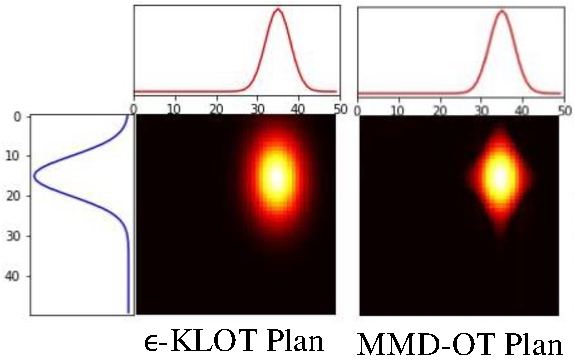
\includegraphics[scale=0.5]{chapter-1/images/synth1.pdf}  
    \caption{}
    %\label{sim1}
\end{subfigure}
\begin{subfigure}{.3\textwidth}
    \centering
    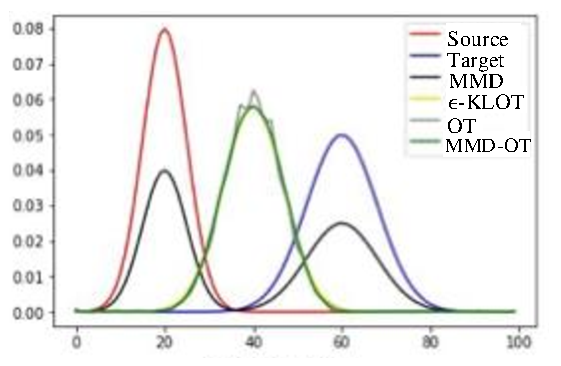
\includegraphics[scale=0.5]{chapter-1/images/synth2.pdf}  
    \caption{}
    %\label{sim1}
\end{subfigure}
\begin{subfigure}{.3\textwidth}
    \centering
    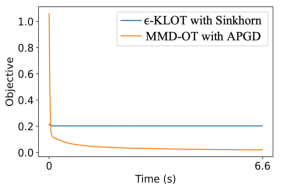
\includegraphics[scale=0.92]{chapter-1/images/synth3.pdf}  
    \caption{}
    %\label{sim1}
\end{subfigure}
\caption[Qualitative comparison of the OT plans and the corresponding barycenters of MMD-OT and related divergences with synthetic Gaussian distributions.]{(a) Optimal Transport plans of $\epsilon$-KLOT and MMD-OT; (b) Barycenter interpolating between Gaussian measures. For the chosen hyperparameter, the barycenters of $\epsilon$-KLOT and MMD-OT overlap and can be looked at as smooth approximations of the OT barycenter; (c) Objective vs Time plot comparing $\epsilon$-KLOT solved using the popular Sinkhorn algorithm~\citep{ChizatPSV18,pham20a}  and MMD-OT~(\ref{eqn:kernot}) solved using APGD. A plot showing $\epsilon$-KLOT's progress at the initial phase is given in Fig.~\ref{time-supp}. 
%More detailed plots are in Figure~\ref{time-supp}.
}\label{fig:planbarytime}
\end{figure}
\paragraph{Visualizing the Level Sets.}
Applications like generative modeling deal with optimization over the parameter (${\theta}$) of the source distribution to match the target distribution. In such cases, it is desirable that the level sets of the distance function over the measures show a lesser number of stationary points that are not global optima~\citep{bottou2017geometrical}. Similar to~\cite{bottou2017geometrical}, we consider a model family for source distributions as
$\mathcal{F} = \{P_{\theta}=\frac{1}{2}(\delta_{\theta}+\delta_{-\theta}):\theta\in[-1,1]\textrm{ x }[-1, 1]\}$ and a fixed target distribution $Q$ as $P_{(2, 2)}\notin \mathcal{F}$. We compute the distances between $P_{\theta}$ and $Q$ according to various divergences.
Fig.~\ref{fig:contours} presents level sets showing the set of distances $\{d(P_{\theta}, Q): \theta\in[-1,1]\textrm{ x }[-1, 1]\}$ where the distance $d(\cdot , \ \cdot)$ is measured using MMD, Kantorovich metric, $\epsilon$-KLOT, and MMD-OT~(9), respectively. 
While all methods correctly identify global minima (green arrow), level sets with MMD-OT and $\epsilon$-KLOT show no local minima (encircled in red for MMD) and have a lesser number of non-optimal stationary points (marked with black arrows) compared to the Kantorovich metric in Fig.~\ref{fig:contours}(b).
\begin{figure*}[t]
    \centering
    \begin{subfigure}{.22\textwidth}
    \centering
    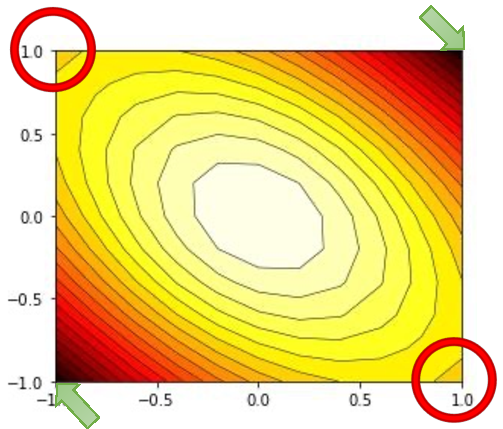
\includegraphics[width=\linewidth]{chapter-1/images/LS1.pdf}  
    \caption{}
    %\label{sim1}
\end{subfigure}
\begin{subfigure}{.22\textwidth}
    \centering
    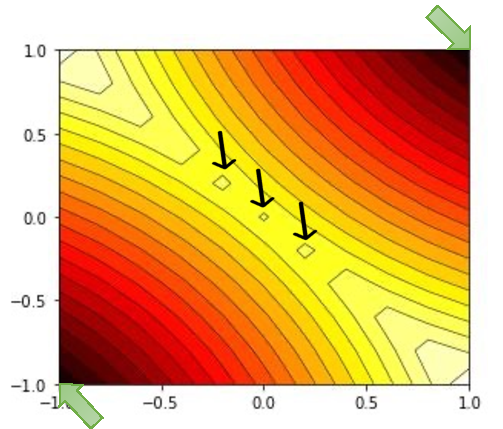
\includegraphics[width=\linewidth]{chapter-1/images/LS2.pdf}  
    \caption{}
    %\label{sim1}
\end{subfigure}
\begin{subfigure}{.22\textwidth}
    \centering
    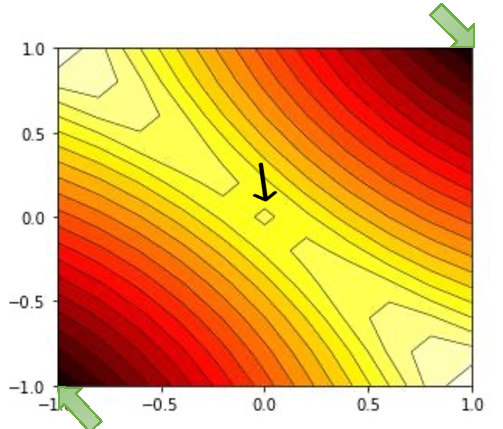
\includegraphics[width=\linewidth]{chapter-1/images/LS3.pdf}  
    \caption{}
    %\label{sim1}
\end{subfigure}
\begin{subfigure}{.22\textwidth}
    \centering
    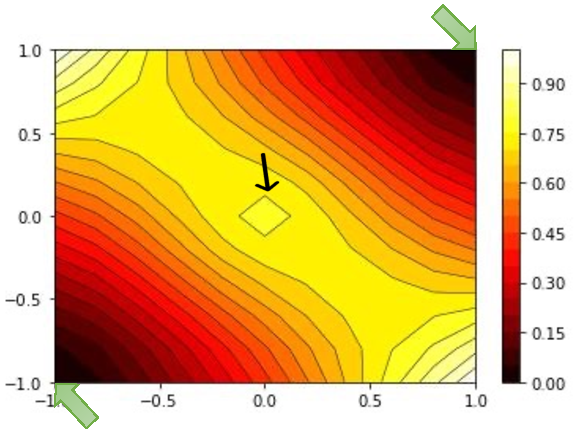
\includegraphics[scale=0.39]{chapter-1/images/LS4.pdf}  
    \caption{}
    %\label{sim1}
\end{subfigure}
    \caption[Qualitative comparison of the level sets of distance function between a family of source distributions and a fixed target distribution of the proposed MMD-OT and related divergences.]{Level sets of distance function between a family of source distributions and a fixed target distribution with the task of finding the source distribution closest to the target distribution using (a) MMD, (b) $\bar{W}_{c, 2}$, (c) $\epsilon$-KLOT, and (d) MMD-OT. 
    While all methods correctly identify global minima (green arrows), level sets with MMD-OT and $\epsilon$-KLOT show no local minima (encircled in red for MMD) and have a lesser number of non-optimal stationary points (marked with black arrows) compared to (b). 
    }
    \label{fig:contours}
\end{figure*}
\paragraph{Computation Time.}
In Fig.~\ref{fig:planbarytime}(c), we present the objective versus time plot. The source and target measures are chosen to be the same, in which case the optimal objective is 0. MMD-OT~(\ref{eqn:kernot}) solved using APGD (Algorithm~\ref{alg:apgd}) gives a much faster rate of decrease in objective compared to the Sinkhorn algorithm used for solving $\epsilon$-KLOT.

\subsection{Two-Sample Hypothesis Test}\label{exp:tst}
Given the sets of samples $\{x_{11}, \dots, x_{1m}\}$ from $ s_0$ and $\{x_{21}, \dots, x_{2m}\}$ from $t_0$, the two-sample test aims to determine whether the two sets of samples are drawn from the same distributions, viz., to predict if $s_0=t_0$. The performance evaluation in the two-sample test relies on two types of errors. Type-I error occurs when $s_0=t_0$, but the test outputs otherwise. Type-II error occurs when the test incorrectly outputs $s_0=t_0$. The probability of Type-I error is called the significance level. The significance level can be controlled using permutation test-based setups~\citep{permutn,dktst}. Algorithms are typically compared based on the empirical estimate of their test power (higher is better), defined as the probability of not making a Type-II error and the average Type-I error (lower is better). 

\paragraph{Experimental Setup.} Following~\cite{dktst}, we consider the two sets of samples, one from the true MNIST~\citep{lecun-mnisthandwrittendigit-2010} and another from fake MNIST generated by the DCGAN~\citep{dcgan}. The data lies in 1024 dimensions. We take an increasing number of samples ($m$) and compute the average test power over 100 pairs of sets for each value of $m$. We repeat the experiment 10 times and report the average test power in Table~\ref{2st-mnist-2} for the significance level $0.05$. By the design of the test, the average Type-I error was upper-bounded, and we noted the Type-II error in our experiment. We detail the procedure for choosing the hyperparameters and the list of chosen hyperparameters for each method in Appendix~\ref{app:tst}.

\paragraph{Results.}
In Table~\ref{2st-mnist-2}, we observe that MMD-OT obtains the highest test power for all values of $m$. The average test power of MMD-OT is $1.5-2.4$ times better than that of $\epsilon$-KLOT across $m$. Our results in the Appendix show that MMD-OT also outperforms EMD and 2-Wasserstein, which suffer from the curse of dimensionality, for all values of $N$. Our results match the sample efficient MMD metric's result on increasing $m$ to 1000, but for a lesser sample size, MMD-OT is always better than MMD.
\begin{table}[t]
\caption[Evaluation of proposed MMD-OT on Two-Sample Hypothesis Test experiment with the MNIST dataset.]{Average Test Power (between 0 and 1; higher is better) on the MNIST dataset with significance level 0.05. MMD-OT obtains the highest average test power at all timesteps.}\label{2st-mnist-2}
% \begin{center}
\centering
\begin{tabular}{cccc}
%\hline
\toprule
$m$ & MMD & $\epsilon$-KLOT & \cellcolor{green!10}{Proposed (MMD-OT)} \\
\midrule
%\hline
100 & 0.137 & 0.099 & \cellcolor{green!10}{\textbf{0.154}}\\
200 & 0.258 & 0.197 & \cellcolor{green!10}{\textbf{0.333}}\\
300 & 0.467 & 0.242 & \cellcolor{green!10}{\textbf{0.588}}\\
400 & 0.656 & 0.324 & \cellcolor{green!10}{\textbf{0.762}}\\
500 & 0.792 & 0.357 & \cellcolor{green!10}{\textbf{0.873}}\\ 
1000 & \textbf{0.909} & 0.506 & \cellcolor{green!10}{\textbf{0.909}}\\ 
%\hline
\bottomrule
\end{tabular}
% \end{center}
\end{table}
\subsection{Single-Cell RNA Sequencing}\label{exp:bary}
We empirically evaluate the quality of our barycenter in the single-cell RNA sequencing experiment. Single-cell RNA sequencing technique (scRNA-seq) helps us understand how the expression profile of the cells changes ~\citep{bioapp19}.
Barycenter estimation in the OT framework offers a principled approach to estimate the trajectory of a measure at an intermediate timestep $t$ ($t_i<t<t_j$) when we have measurements available only at $t_i$ (source) and $t_j$ (target) time steps (Fig.~\ref{fig:CPD}).
\begin{figure}[t]
    \centering
    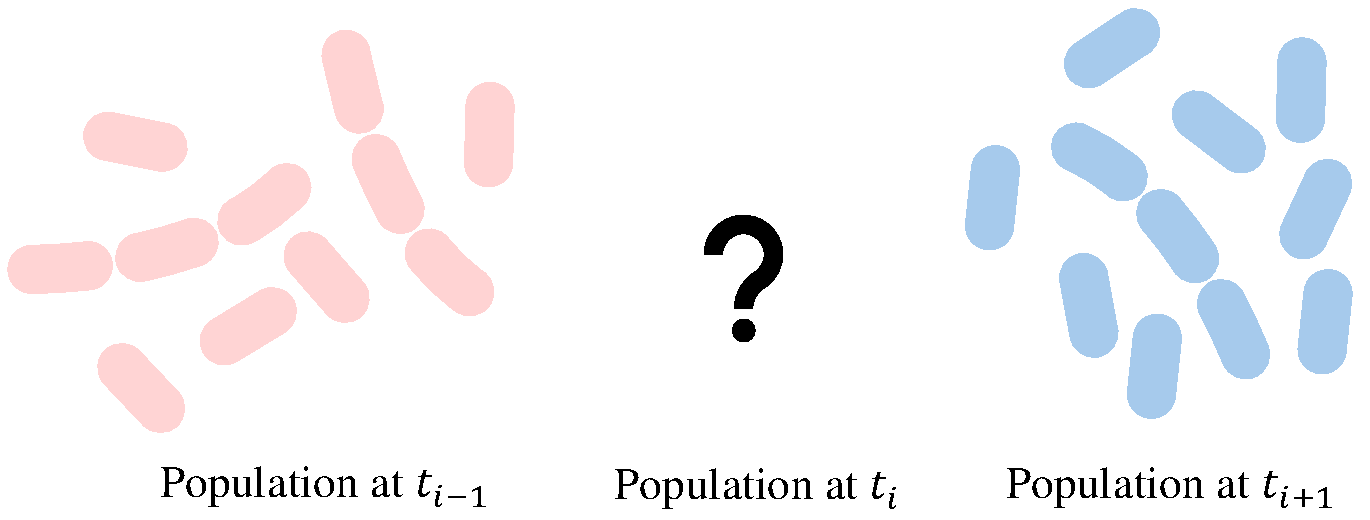
\includegraphics[width=0.5\linewidth]{chapter-1/images/CPD.pdf}
    \caption[Illustration of the single-cell RNA sequencing experimental setup.]{Illustration of the single-cell RNA sequencing experimental setup.}
    \label{fig:CPD}
\end{figure}

\paragraph{Experimental Setup.}
We perform experiments on the Embryoid Body (EB) single-cell dataset~\citep{moon19a}. The dataset has samples available at five timesteps ($t_j$ with $j=0,\ldots,4$), which were collected during a 25-day period of development of the human embryo. Following~\cite{TNet20}, we project the data onto two-dimensional space and associate uniform measures to the source and the target samples given at different timesteps. 
We consider the samples at timestep $t_i$ and $t_{i+2}$ as the samples from the source and target measures where $0\leq i \leq 2$ and aim at estimating the measure at $t_i$ timestep as their barycenter with equal interpolation weights $\rho_1 = \rho_2 = 0.5$. 

We compute the barycenters using MMD-OT (\ref{eqn:baryker}) and the $\epsilon$-KLOT~\citep{chizat18a,Liero2018} approaches. 
For both, a simplex constraint is used to cater to the case of uniform measures. We also compare against the empirical average of the source and target measures, which is the barycenter obtained with the MMD metric. 
The computed barycenter is evaluated against the measure corresponding to the ground truth samples available at the corresponding timestep. We compute the distance between the two using the MMD metric with RBF kernel~\citep{gretton12a}. %and sigma-heuristic~\citep{gretton12a}. 
The hyperparameters are chosen based on the leave-one-out validation protocol. More details and some additional results are in Appendix~\ref{appendix:scrna}.
\begin{table}[t]
\caption[Evaluation of the interpolating barycenter of MMD-OT on Single-Cell RNA Sequencing experiment.]{MMD distance (lower is better) between computed barycenter and the ground truth distribution. A sigma-heuristics based RBF kernel is used to compute the MMD distance. We observe that MMD-OT's results are closer to the ground truth than the baselines' results at all timesteps.}
\label{table:mmd-bio}
% \begin{center}
\centering
\begin{tabular}{cccc}
\toprule
Timestep &  MMD & $\epsilon$-KLOT & \cellcolor{green!10}{Proposed (MMD-OT)}\\
\midrule
$t_1$ & 0.375 & 0.391 & \cellcolor{green!10}{\textbf{0.334}}\\
$t_2$ & 0.190 & 0.184 & \cellcolor{green!10}{\textbf{0.179}}\\
$t_3$ & 0.125 & 0.138 & \cellcolor{green!10}{\textbf{0.116}}\\
\midrule
Avg. & 0.230 & 0.238 & \cellcolor{green!10}{\textbf{0.210}}\\
\bottomrule
\end{tabular}
% \end{center}
\end{table}

\paragraph{Results.}
Table~\ref{table:mmd-bio} shows that MMD-OT achieves the lowest distance from the ground truth for all the timesteps, illustrating its superior interpolation performance. 
\subsection{Domain Adaptation}\label{jumbot-mnist}
OT has been widely employed in domain adaptation problems~\citep{Courty17domAda,courty17b,seguy2018large,damodaran2018deepjdot}. JUMBOT~\citep{jumbot} is a recent framework for the task of unsupervised domain adaptation (UDA). JUMBOT is based on $\epsilon$-KLOT that outperforms OT-based baselines.
JUMBOT's loss function involves a cross-entropy term and $\epsilon$-KLOT discrepancy term between the source and target distributions as shown in Fig.~\ref{fig:UDA-illus}. We showcase the utility of MMD-OT  (\ref{eqn:kernot}) in the JUMBOT~\citep{jumbot} framework.

\begin{table}[t]
\caption[Evaluation of proposed MMD-OT on the domain adaptation experiment with the MNIST dataset.]{Target domain accuracy (higher is better) obtained in domain adaptation experiments. Results for $\epsilon$-KLOT are reproduced from the code open-sourced for JUMBOT in~\cite{jumbot}. MMD-OT outperforms $\epsilon$-KLOT in all the domain adaptation tasks considered.}
\label{DA-main}
% \begin{center}
\centering
\begin{tabular}{cccc}
\toprule
Source & Target & JUMBOT \citep{jumbot} & \cellcolor{green!10}{Proposed}\\
& & ($\epsilon$-KLOT) & \cellcolor{green!10}{(MMD-OT)} \\
\midrule
M-MNIST & USPS & 91.53 & \cellcolor{green!10}{\textbf{94.97}}\\
M-MNIST & MNIST & 99.35 & \cellcolor{green!10}{\textbf{99.50}}\\
MNIST & M-MNIST & 96.51 & \cellcolor{green!10}{\textbf{96.96}}\\
MNIST & USPS & 96.51 & \cellcolor{green!10}{\textbf{97.01}}\\
SVHN & M-MNIST & 94.26 & \cellcolor{green!10}{\textbf{95.35}}\\
SVHN & MNIST & 98.68 & \cellcolor{green!10}{\textbf{98.98}}\\
SVHN & USPS & 92.78 & \cellcolor{green!10}{\textbf{93.22}}\\
USPS & MNIST & 96.76 & \cellcolor{green!10}{\textbf{98.53}}\\
\midrule
\multicolumn{2}{c}{Avg.} & 95.80 & \textbf{96.82} \\
\bottomrule
\end{tabular}
% \end{center}
\end{table}

\paragraph{Experimental Setup.} We first evaluate the performance of MMD-OT in the JUMBOT framework on the Digits datasets comprising MNIST~\citep{lecun-mnisthandwrittendigit-2010}, M-MNIST~\citep{mmnist-ganin2016domain}, SVHN~\citep{svhn}, USPS~\citep{usps} datasets. We replace the $\epsilon$-KLOT based loss with the MMD-OT loss (\ref{eqn:kernot}), keeping the other experimental set-up the same as JUMBOT. We obtain JUMBOT's result with $\epsilon$-KLOT with the best-reported hyperparameters~\citep{jumbot}. Following JUMBOT, we tune hyperparameters of MMD-OT for the Digits experiment on USPS to MNIST (U$\mapsto$M) domain adaptation task and use the same hyperparameters for the rest of the domain adaptation tasks on Digits. More details are in Appendix~\ref{app:jumbot}. 
\begin{figure}[t]
    \centering
    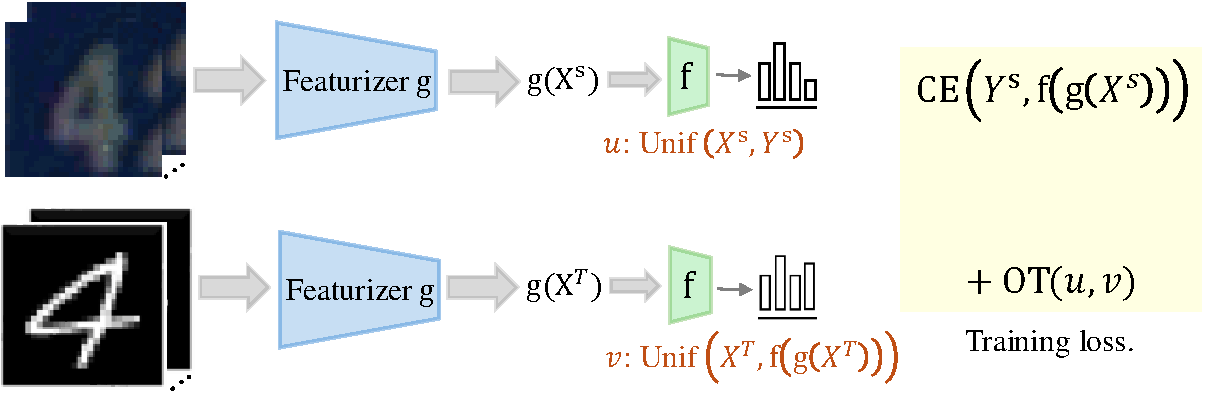
\includegraphics[width=0.8\linewidth]{chapter-1/images/UDA-illus.pdf}
    \caption[Illustration of the setup for domain adaptation experiment.]{Illustration of the setup for domain adaptation experiment. CE denotes the cross entropy loss. S and T denote the source and target domains, respectively. Unif($X, Y$) represents the Uniform distribution over the set of input-label samples.}
    \label{fig:UDA-illus}
\end{figure}
\paragraph{Results.} Table~\ref{DA-main} reports the accuracy obtained on target datasets. We observe that MMD-OT-based loss performs better than $\epsilon$-KLOT-based loss for all the domain adaptation tasks. In Fig.~\ref{tsne}, we also compare the t-SNE plot of the embeddings learned with the MMD-OT and the $\epsilon$-KLOT-based loss functions. The clusters learned with  MMD-OT are better separated (e.g., red- and cyan-colored clusters).


With superior results on the Digits dataset, we evaluate MMD-OT on larger datasets for domain adaptation. We also include other popular domain adaptation baselines having ResNet-50 backbone as in JUMBOT \citep{jumbot}. These include DANN~\citep{mmnist-ganin2016domain}, CDANN-E~\citep{Long2017ConditionalAD}, 
ALDA~\citep{Chen2020AdversarialLearnedLF},
DEEPJDOT~\citep{damodaran2018deepjdot}, ROT~\citep{ROT}, and BombOT~\citep{bomb-ot}. BombOT is a recent state-of-the-art OT-based method for unsupervised domain adaptation (UDA). As in JUMBOT~\citep{jumbot}, BombOT also employs $\epsilon$-KLOT based loss function. 
We also include the results of the baseline ResNet-50 model, where the model is trained on the source and is evaluated on the target without employing any adaptation techniques.

\begin{table}[t]
    \caption[Evaluation (task-wise) of MMD-OT on the unsupervised domain adaptation experiment with the Office-Home dataset.]{Target accuracies (higher is better) on the Office-Home dataset in the UDA setting. The letters denote different domains: `A' for Artistic images, `P' for Product images, `C' for Clip art and `R' for Real-World images. The proposed method achieves the highest accuracy on almost all the domain adaptation tasks. 
    % It is worth noting that the proposed method, which is based on the JUMBOT framework, achieves better results even when compared to the $\epsilon$KL-UOT result based on the BombOT framework~\citep{bomb-ot}. The BombOT framework additionally incorporates the interaction between the minibatches. For a more direct comparison of the divergences (excluding the effect of minibatch interaction), we implement our method in the JUMBOT framework. 
    }\label{office-home}
    \setlength{\tabcolsep}{1.5pt}
    % \begin{center}
    \centering
    \begin{footnotesize}
    \begin{tabular}{lcccccccccccc}
    \toprule
       Method & 
       A$\rightarrow$C&%\tiny{\textbf{A}}$\rightarrow$\tiny{\textbf{C}} & 
       A$\rightarrow$P&%\tiny{\textbf{A}}$\rightarrow$\tiny{\textbf{P}} & 
       A$\rightarrow$R&%\tiny{\textbf{A}}$\rightarrow$\tiny{\textbf{R}} & 
       C$\rightarrow$A&%\tiny{\textbf{C}}$\rightarrow$\tiny{\textbf{A}} & 
       C$\rightarrow$P&%\tiny{\textbf{C}}$\rightarrow$\tiny{\textbf{P}} & 
       C$\rightarrow$R&%\tiny{\textbf{C}}$\rightarrow$\tiny{\textbf{R}} & 
       P$\rightarrow$A&%\tiny{\textbf{P}}$\rightarrow$\tiny{\textbf{A}} & 
       P$\rightarrow$C&%\tiny{\textbf{P}}$\rightarrow$\tiny{\textbf{C}} & 
       P$\rightarrow$R&%\tiny{\textbf{P}}$\rightarrow$\tiny{\textbf{R}} & 
       R$\rightarrow$A&%\tiny{\textbf{R}}$\rightarrow$\tiny{\textbf{A}} & 
       R$\rightarrow$C&%\tiny{\textbf{R}}$\rightarrow$\tiny{\textbf{C}} & 
       R$\rightarrow$P\\
       \midrule
       ResNet-50 & 34.9 & 50.0 & 58.0 & 37.4 & 41.9 & 46.2 & 38.5 & 31.2 & 60.4 & 53.9 & 41.2 & 59.9\\
       \midrule
       DANN & \multirow{2}{*}{44.3} & \multirow{2}{*}{59.8} & \multirow{2}{*}{69.8} & \multirow{2}{*}{48.0}  & \multirow{2}{*}{58.3} & \multirow{2}{*}{63.0} & \multirow{2}{*}{49.7}  & \multirow{2}{*}{42.7} & \multirow{2}{*}{70.6} & \multirow{2}{*}{64.0} & \multirow{2}{*}{51.7} & \multirow{2}{*}{78.3} \\
       \citep{mmnist-ganin2016domain}\\
       \midrule
       CDAN-E & \multirow{2}{*}{52.5} & \multirow{2}{*}{71.4} & \multirow{2}{*}{76.1} & \multirow{2}{*}{59.7}  & \multirow{2}{*}{69.9} & \multirow{2}{*}{71.5} & \multirow{2}{*}{58.7}  & \multirow{2}{*}{50.3} & \multirow{2}{*}{77.5} & \multirow{2}{*}{70.5} & \multirow{2}{*}{57.9} & \multirow{2}{*}{83.5} \\ 
       \citep{Long2017ConditionalAD}\\
       \midrule
       DEEPJDOT & \multirow{2}{*}{50.7} &  \multirow{2}{*}{68.7} & \multirow{2}{*}{74.4} & \multirow{2}{*}{59.9}  & \multirow{2}{*}{65.8} & \multirow{2}{*}{68.1} & \multirow{2}{*}{55.2}  & \multirow{2}{*}{46.3} & \multirow{2}{*}{73.8} & \multirow{2}{*}{66.0} & \multirow{2}{*}{54.9} & \multirow{2}{*}{78.3} \\
       \citep{damodaran2018deepjdot}\\
       \midrule
       ALDA & \multirow{2}{*}{52.2} & \multirow{2}{*}{69.3} & \multirow{2}{*}{76.4} & \multirow{2}{*}{58.7}  & \multirow{2}{*}{68.2} & \multirow{2}{*}{71.1} & \multirow{2}{*}{57.4} & \multirow{2}{*}{49.6} & \multirow{2}{*}{76.8} & \multirow{2}{*}{70.6} & \multirow{2}{*}{57.3} & \multirow{2}{*}{82.5} \\
       \citep{Chen2020AdversarialLearnedLF}\\
       \midrule
       ROT & \multirow{2}{*}{47.2} & \multirow{2}{*}{71.8} & \multirow{2}{*}{76.4} & \multirow{2}{*}{58.6}  & \multirow{2}{*}{68.1} & \multirow{2}{*}{70.2} & \multirow{2}{*}{56.5}  & \multirow{2}{*}{45.0} & \multirow{2}{*}{75.8} & \multirow{2}{*}{69.4} & \multirow{2}{*}{52.1} & \multirow{2}{*}{80.6} \\
       \citep{ROT}\\
       \midrule
       $\epsilon$-KLOT (JUMBOT) & \multirow{2}{*}{55.2} & \multirow{2}{*}{75.5} & \multirow{2}{*}{80.8} & \multirow{2}{*}{65.5}  & \multirow{2}{*}{74.4} & \multirow{2}{*}{74.9} & \multirow{2}{*}{65.2}  & \multirow{2}{*}{52.7} & \multirow{2}{*}{79.2} & \multirow{2}{*}{73.0} & \multirow{2}{*}{59.9} & \multirow{2}{*}{83.4}\\
       \citep{jumbot}\\
       \midrule
       BombOT & \multirow{2}{*}{56.2} & \multirow{2}{*}{75.2} & \multirow{2}{*}{80.5} & \multirow{2}{*}{65.8}  & \multirow{2}{*}{74.6} & \multirow{2}{*}{75.4} & \multirow{2}{*}{66.2}  & \multirow{2}{*}{53.2} & \multirow{2}{*}{80.0} & \multirow{2}{*}{74.2} & \multirow{2}{*}{\textbf{60.1}} & \multirow{2}{*}{83.3} \\
       \citep{bomb-ot}\\
       \midrule
       \cellcolor{green!10}{Proposed (MMD-OT)} & \cellcolor{green!10}{\textbf{56.5}} & \cellcolor{green!10}{\textbf{77.2}} & \cellcolor{green!10}{\textbf{82.0}} & \cellcolor{green!10}{\textbf{70.0}}  & \cellcolor{green!10}{\textbf{77.1}} & \cellcolor{green!10}{\textbf{77.8}} & \cellcolor{green!10}{\textbf{69.3}}  & \cellcolor{green!10}{\textbf{55.1}} & \cellcolor{green!10}{\textbf{82.0}} & \cellcolor{green!10}{\textbf{75.5}} & \cellcolor{green!10}{59.3} & \cellcolor{green!10}{\textbf{84.0}}\\
        \bottomrule
    \end{tabular}
    \end{footnotesize}
    % \end{center}
\end{table}

\begin{table}[ht!]
{
\caption[Evaluation (average-score-wise) of MMD-OT on the unsupervised domain adaptation experiment with the Office-Home dataset.]{Average target accuracies (higher is better) on the Office-Home dataset in the UDA setting. The proposed MMD-OT method achieves the highest accuracy.}\label{office-home-avg}
% \begin{center}
\begin{tabular}{ccccccccc}
\toprule
ResNet-50 & DANN & CDAN-E & DEEPJDOT & ALDA & ROT & $\epsilon$-KLOT & BombOT & \cellcolor{green!10}{MMD-OT}\\
\midrule
 46.1 & 58.3 & 66.6 & 63.5 & 65.8 & 64.3 & 70.0 & 70.4 & \cellcolor{green!10}{\textbf{72.0}} \\
\bottomrule
\end{tabular}
}
\end{table}

% \begin{table}
%     \caption{Target accuracies (higher is better) on the Office-Home dataset in the UDA setting. The letters denote different domains: `A' for Artistic images, `P' for Product images, `C' for Clip art and `R' for Real-World images. The proposed method achieves the highest accuracy on almost all the domain adaptation tasks and achieves the best accuracy averaged across the tasks. 
%     }\label{office-home}
%     \setlength{\tabcolsep}{4pt}
%     \begin{center}
%     \begin{footnotesize}
%     \begin{tabular}{lccccccccc}
%     \toprule
%        \textbf{Method} & 
%        A$\rightarrow$C&%\tiny{\textbf{A}}$\rightarrow$\tiny{\textbf{C}} & 
%        A$\rightarrow$P&%\tiny{\textbf{A}}$\rightarrow$\tiny{\textbf{P}} & 
%        A$\rightarrow$R&%\tiny{\textbf{A}}$\rightarrow$\tiny{\textbf{R}} & 
%        C$\rightarrow$A&%\tiny{\textbf{C}}$\rightarrow$\tiny{\textbf{A}} & 
%        C$\rightarrow$P&%\tiny{\textbf{C}}$\rightarrow$\tiny{\textbf{P}} & 
%        C$\rightarrow$R&%\tiny{\textbf{C}}$\rightarrow$\tiny{\textbf{R}} & 
%        P$\rightarrow$A&%\tiny{\textbf{P}}$\rightarrow$\tiny{\textbf{A}} & 
%        P$\rightarrow$C&%\tiny{\textbf{P}}$\rightarrow$\tiny{\textbf{C}} & 
%        P$\rightarrow$R
%        \\
%        \midrule
%        ResNet-50 & 34.9 & 50.0 & 58.0 & 37.4 & 41.9 & 46.2 & 38.5 & 31.2 & 60.4\\
%        \midrule
%        DANN & \multirow{2}{*}{44.3} & \multirow{2}{*}{59.8} & \multirow{2}{*}{69.8} & \multirow{2}{*}{48.0}  & \multirow{2}{*}{58.3} & \multirow{2}{*}{63.0} & \multirow{2}{*}{49.7}  & \multirow{2}{*}{42.7} & \multirow{2}{*}{70.6}\\
%        \citep{Ganin2015DomainAdversarialTO}\\
%        \midrule
%        CDAN-E & \multirow{2}{*}{52.5} & \multirow{2}{*}{71.4} & \multirow{2}{*}{76.1} & \multirow{2}{*}{59.7}  & \multirow{2}{*}{69.9} & \multirow{2}{*}{71.5} & \multirow{2}{*}{58.7}  & \multirow{2}{*}{50.3} & \multirow{2}{*}{77.5}\\ 
%        \citep{Long2017ConditionalAD}\\
%        \midrule
%        DEEPJDOT & \multirow{2}{*}{50.7} &  \multirow{2}{*}{68.7} & \multirow{2}{*}{74.4} & \multirow{2}{*}{59.9}  & \multirow{2}{*}{65.8} & \multirow{2}{*}{68.1} & \multirow{2}{*}{55.2}  & \multirow{2}{*}{46.3} & \multirow{2}{*}{73.8}\\
%        \citep{damodaran2018deepjdot}\\
%        \midrule
%        ALDA & \multirow{2}{*}{52.2} & \multirow{2}{*}{69.3} & \multirow{2}{*}{76.4} & \multirow{2}{*}{58.7}  & \multirow{2}{*}{68.2} & \multirow{2}{*}{71.1} & \multirow{2}{*}{57.4} & \multirow{2}{*}{49.6} & \multirow{2}{*}{76.8}\\
%        \citep{Chen2020AdversarialLearnedLF}\\
%        \midrule
%        ROT & \multirow{2}{*}{47.2} & \multirow{2}{*}{71.8} & \multirow{2}{*}{76.4} & \multirow{2}{*}{58.6}  & \multirow{2}{*}{68.1} & \multirow{2}{*}{70.2} & \multirow{2}{*}{56.5}  & \multirow{2}{*}{45.0} & \multirow{2}{*}{75.8}\\
%        \citep{ROT}\\
%        \midrule
%        $\epsilon$-KLOT (JUMBOT) & \multirow{2}{*}{55.2} & \multirow{2}{*}{75.5} & \multirow{2}{*}{80.8} & \multirow{2}{*}{65.5}  & \multirow{2}{*}{74.4} & \multirow{2}{*}{74.9} & \multirow{2}{*}{65.2}  & \multirow{2}{*}{52.7} & \multirow{2}{*}{79.2}\\
%        \citep{jumbot}\\
%        \midrule
%        BombOT & \multirow{2}{*}{56.2} & \multirow{2}{*}{75.2} & \multirow{2}{*}{80.5} & \multirow{2}{*}{65.8}  & \multirow{2}{*}{74.6} & \multirow{2}{*}{75.4} & \multirow{2}{*}{66.2}  & \multirow{2}{*}{53.2} & \multirow{2}{*}{80.0}\\
%        \citep{bomb-ot}\\
%        \midrule
%        Proposed & \textbf{56.5} & \textbf{77.2} & \textbf{82.0} & \textbf{70.0}  & \textbf{77.1} & \textbf{77.8} & \textbf{69.3}  & \textbf{55.1} & \textbf{82.0}\\
%         \bottomrule
%     \end{tabular}
%     \end{footnotesize}
%     \end{center}
% \end{table}
% \begin{table}
%     \caption{Target accuracies (higher is better) on the Office-Home dataset in the UDA setting. The letters denote different domains: `A' for Artistic images, `P' for Product images, `C' for Clip art and `R' for Real-World images. The proposed method achieves the highest accuracy on almost all the domain adaptation tasks and achieves the best accuracy averaged across the tasks. 
%     }\label{office-home2}
%     \setlength{\tabcolsep}{4pt}
%     \begin{center}
%     \begin{footnotesize}
%     \begin{tabular}{lcccl}
%     \toprule
%        Method & 
%        R$\rightarrow$A&%\tiny{\textbf{R}}$\rightarrow$\tiny{\textbf{A}} & 
%        R$\rightarrow$C&%\tiny{\textbf{R}}$\rightarrow$\tiny{\textbf{C}} & 
%        R$\rightarrow$P&%\tiny{\textbf{R}}$\rightarrow$\tiny{\textbf{P}} & 
%        \textbf{Avg}\\
%        \midrule
%        ResNet-50 &  53.9 & 41.2 & 59.9 & 46.1\\
%        \midrule
%        DANN & \multirow{2}{*}{64.0} & \multirow{2}{*}{51.7} & \multirow{2}{*}{78.3} & \multirow{2}{*}{58.3}\\
%        \citep{Ganin2015DomainAdversarialTO}\\
%        \midrule
%        CDAN-E & \multirow{2}{*}{70.5} & \multirow{2}{*}{57.9} & \multirow{2}{*}{83.5} & \multirow{2}{*}{66.6}\\ 
%        \citep{Long2017ConditionalAD}\\
%        \midrule
%        DEEPJDOT & \multirow{2}{*}{66.0} & \multirow{2}{*}{54.9} & \multirow{2}{*}{78.3} & \multirow{2}{*}{63.5}\\
%        \citep{damodaran2018deepjdot}\\
%        \midrule
%        ALDA & \multirow{2}{*}{70.6} & \multirow{2}{*}{57.3} & \multirow{2}{*}{82.5} & \multirow{2}{*}{65.8}\\
%        \citep{Chen2020AdversarialLearnedLF}\\
%        \midrule
%        ROT & \multirow{2}{*}{69.4} & \multirow{2}{*}{52.1} & \multirow{2}{*}{80.6} & \multirow{2}{*}{64.3}\\
%        \citep{ROT}\\
%        \midrule
%        $\epsilon$-KLOT (JUMBOT) &  \multirow{2}{*}{73.0} & \multirow{2}{*}{59.9} & \multirow{2}{*}{83.4} & \multirow{2}{*}{70.0}\\
%        \citep{jumbot}\\
%        \midrule
%        BombOT & \multirow{2}{*}{74.2} & \multirow{2}{*}{\textbf{60.1}} & \multirow{2}{*}{83.3} & \multirow{2}{*}{70.4}\\
%        \citep{bomb-ot}\\
%        \midrule
%        Proposed  & \textbf{75.5} & 59.3 & \textbf{84.0} & \textbf{72.2}\\
%         \bottomrule
%     \end{tabular}
%     \end{footnotesize}
%     \end{center}
% \end{table}

{On Office-Home Dataset:} We evaluate the proposed method on the Office-Home dataset~\citep{venkateswara2017deep}, popular for unsupervised domain adaptation. We use the backbone network of ResNet-50 following. The Office-Home dataset has 15,500 images from four domains: Artistic images (A), Clip
Art (C), Product images (P) and Real-World (R). The dataset contains images of 65 object categories
common in office and home scenarios for each domain. Following~\cite{jumbot, bomb-ot}, evaluation is done in 12 adaptation tasks. Following JUMBOT, we validate the proposed method on the A$\rightarrow$C task and use the chosen hyperparameters for the rest of the tasks.

Tables~\ref{office-home} and \ref{office-home-avg} report the target accuracies obtained by different methods. The results of the BombOT method are quoted from \cite{bomb-ot}, and the results of other baselines are quoted from~\cite{jumbot}. We observe that the proposed MMD-OT-based method achieves the best target accuracy in $11$ out of $12$ adaptation tasks and obtains the best average accuracy.

{On VisDA-2017 Dataset:} We now consider the next domain adaptation task between the training and validation sets of the VisDA-2017~\citep{Recht2018DoCC} dataset. We follow the experimental setup detailed in \cite{jumbot}. The source domain of VisDA has 152,397 synthetic images, while the target domain has 55,388 real-world images. Both the domains have 12 object categories. 

Table~\ref{visda} compares the performance of different methods. 
The results of the BombOT method are quoted from \cite{bomb-ot}, and the results of other baselines are quoted from~\cite{jumbot}.
The proposed method achieves the best performance, improving the accuracy obtained by $\epsilon$-KLOT based JUMBOT and BombOT methods by $4.5\%$ and $2.4\%$, respectively.

\begin{table}
\caption[Evaluation of proposed MMD-OT on the unsupervised domain adaptation experiment with the VisDA-2017 dataset.]{Target accuracies (higher is better) on the VisDA-2017 dataset in the UDA setting. The proposed MMD-OT method achieves the highest accuracy.}\label{visda}
% \begin{center}
\centering
\begin{tabular}{cccccccc}
\toprule
Dataset & CDAN-E & ALDA & DEEPJDOT & ROT & $\epsilon$-KLOT & BombOT & \cellcolor{green!10}{MMD-OT}\\
\midrule
 VisDA-2017 & 70.1 & 70.5 & 68.0 & 66.3 & 72.5 & 74.6 & \cellcolor{green!10}{\textbf{77.0}} \\
\bottomrule
\end{tabular}
% \end{center}
\end{table}
\subsection{Prompt Learning for Few-Shot Classification}\label{exp:prompt-uot}
The task of learning prompts (e.g. ``a tall bird of [class]'') for vision-language models has emerged as a promising approach to adapt large pre-trained models like CLIP~\citep{clip} for downstream tasks. The similarity between prompt features (which are class-specific) and visual features of a given image can help us classify the image. A recent OT-based prompt learning approach, PLOT~\citep{chen2023plot}, obtained state-of-the-art results on the $\mathcal{F}$-shot recognition task in which only $\mathcal{F}$ images per class are available during training. Fig.~\ref{fig:prompt-illus} shows the setup of this experiment.
\paragraph{Experimental Setup.}
We evaluate the performance of MMD-OT following the setup of~\cite{chen2023plot} on the benchmark EuroSAT~\citep{helber2019eurosat} dataset consisting of satellite images, DTD~\citep{dtd} dataset having images of textures and Oxford-Pets~\citep{oxp} dataset having images of pets. 
\begin{figure}[t]
    \centering
    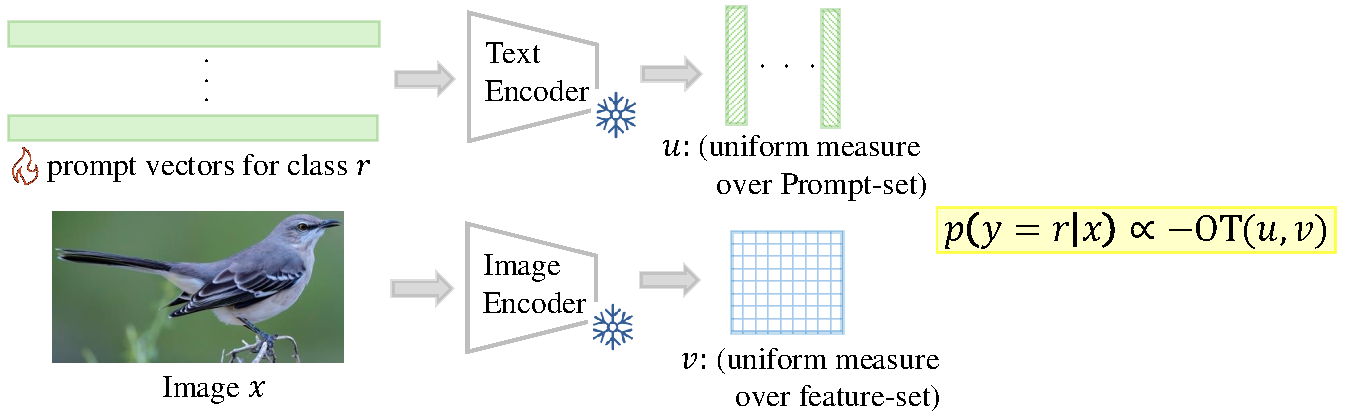
\includegraphics[width=\linewidth]{chapter-1/images/prompt-illustr.pdf}
    \caption[Illustration of the setup for the task of learning prompts for few-shot classification.]{Illustration of the setup for the task of learning prompts for few-shot classification. Figure adapted from \cite{chen2023plot}.}
    \label{fig:prompt-illus}
\end{figure}

\begin{table*}[ht!]
\caption[Evaluation of proposed MMD-OT on the prompt learning experiment for few-shot classification.]{Average and standard deviation (over 3 runs) of accuracy (higher is better) on the $\mathcal{F}$-shot classification task, shown for different values of shots ($\mathcal{F}$) in the state-of-the-art PLOT framework. The proposed method replaces OT with MMD-OT in PLOT, keeping all other hyperparameters the same. The results of PLOT are taken from their paper~\citep{chen2023plot}.} \label{tableplot} 
% \begin{center}
\centering
\footnotesize{
\begin{tabular}{llccccc}
\toprule
Dataset & Method & 1 & 2 & 4 & 8 & 16 \\
\midrule
\multirow{ 2}{*}{EuroSAT} & PLOT & 54.05 $\pm$ 5.95 & 64.21 $\pm$ 1.90 & \textbf{72.36} $\pm$ \textbf{2.29} & 78.15 $\pm$ 2.65 & 82.23 $\pm$ 0.91 \\ 
 & \cellcolor{green!10}{Proposed} & \cellcolor{green!10}{\textbf{58.47} $\pm$ \textbf{1.37}} & \cellcolor{green!10}{\textbf{66.0} $\pm$ \textbf{0.93}} & \cellcolor{green!10}{71.97 $\pm$ 2.21} & \cellcolor{green!10}{\textbf{79.03} $\pm$ \textbf{1.91}} & \cellcolor{green!10}{\textbf{83.23} $\pm$ \textbf{0.24}}\\ 
\midrule
\multirow{ 2}{*}{DTD} & PLOT & 46.55 $\pm$ 2.62 & \textbf{51.24} $\pm$ \textbf{1.95} & 56.03 $\pm$ 0.43  & 61.70 $\pm$ 0.35 & 65.60 $\pm$ 0.82\\ 
 & \cellcolor{green!10}{Proposed} & \cellcolor{green!10}{\textbf{47.27}$\pm$\textbf{1.46}} & \cellcolor{green!10}{51.0$\pm$1.71} & \cellcolor{green!10}{\textbf{56.40}$\pm$\textbf{0.73}} & \cellcolor{green!10}{\textbf{63.17}$\pm$\textbf{0.69}} & \cellcolor{green!10}{\textbf{65.90} $\pm$ \textbf{0.29}}\\ 
 \bottomrule
\end{tabular}}
% \end{center}
\end{table*}

\paragraph{Results.} With the same evaluation protocol as in~\cite{chen2023plot}, we report the classification accuracy averaged over three seeds in Table~\ref{tableplot}. We note that MMD-OT-based prompt-learning achieves better results than PLOT, especially when $\calF$ is less (more challenging case due to lesser training data). With the EuroSAT dataset, the improvement is as high as 4\% for a challenging case of $\mathcal{F}$=1. More details are in Appendix~\ref{app:prompt}. 

\section{Conclusion}\label{sec:conclusion}
The literature on regularized variants of OT has largely focused on $f$-divergence-based regularization. Our work provides a comprehensive analysis of MMD-regularization in OT, answering many open questions. We prove novel theoretical results on the metricity and the sample efficiency of MMD-OT, propose consistent estimators which can be computed efficiently, and illustrate its empirical effectiveness in several applications. Our theoretical and empirical contributions for MMD-OT and its corresponding barycenter demonstrate the potential of MMD-regularization in OT  as an effective alternative to $f$-divergence-based regularization. 
